\section{Dualshock4 Treiber (Becker)}

Gemäß der Anforderung ist die Steuerung des Fahrzeugs sowie der Geschützplattform durch einen DualShock4-Controller vorgesehen. 
Einerseits dient dies dem Testen der Plattformsteuerung für den späteren Betrieb der KI. 
Des Weiteren fungiert sie als Gamification-Element. 
Das Ziel ist die Steigerung des Nutzens und der Freude an dem Projekt, indem eine bekannte Steuerungsmethode verwendet wird, welche die Benutzerfreundlichkeit erhöht.

Für die Realisierung dieser Funktionalität wurde ein spezieller Treiber entwickelt, der den Zustand des Controllers in regelmäßigen Abständen an den ESP-32 übermittelt. 
Darüber hinaus umfasste mein Wunsch eine Funktion, die Vibrationen und Farbwechsel am Gamepad auslöst, und zwar vom Mikrocontroller aus.

\subsection{Übertragung}

Vor jeglicher Datenübertragung muss zunächst eine Kopplung per Bluetooth hergestellt werden. 
Der Sony Dualshock 4 Controller verwendet in diesem Fall den Bluetooth Classic 4.0 Standard.
Für die Verbindung des Controllers mit den Geräten ist im Flash-Speicher des Gamepads eine MAC-Adresse gespeichert. 
Beim Anschalten des Controllers wird versucht, Kontakt zu dieser Adresse aufzubauen.
Unter normalen Betriebsbedingungen wäre dies die Adresse der PlayStation4-Konsole. 
Für unser Projekt wurde jedoch die gespeicherte MAC-Adresse mit der des ESP-32 überschrieben.
Nach dem Einschalten unternimmt das Gamepad sofort den Versuch, sich mit dem Mikrocontroller zu verbinden.

Die Übertragung der Daten zwischen Gamepad und Mikrocontroller erfolgt mittels sogenannter HID-Reports.
HID-Reports sind binäre Datenstrukturen, welche die Reihenfolge der Informationen festlegen.
Die Struktur der Reports wurde von Sony nicht öffentlich zur Verfügung gestellt. 
Allerdings war es einigen Personen möglich, durch Reverse-Engineering wichtige Felder zu ermitteln \cite{esp_ds4_hid_reports}.

Das Human Interface Device (HID)-Protokoll ist ein standardisiertes Kommunikationsprotokoll zur Übertragung von Eingabe- und Steuerdaten zwischen Peripheriegeräten (z.B. Tastaturen, Mäusen, Gamepads) und einem Host-System. 
Es wurde ursprünglich für USB spezifiziert \cite{esp_usb_hid_spec} und später für Bluetooth Classic übernommen.

\begin{figure}[ht]
    \centering
    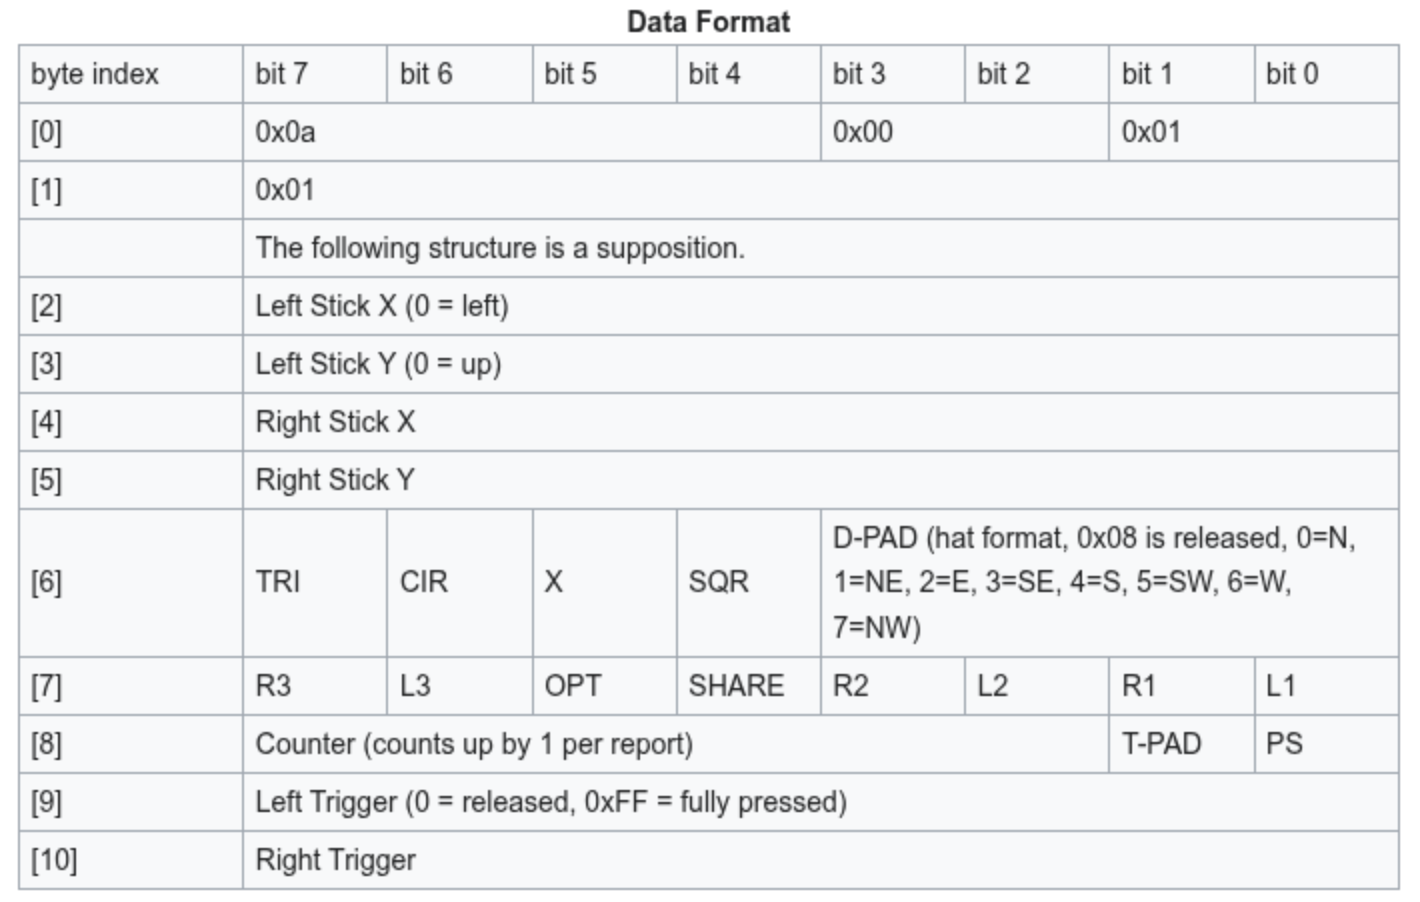
\includegraphics[width=0.7\textwidth]{images/becker_esp32_ds4_report.png}
    \caption{Beispielhafter Aufbau eines HID-Reports aus \cite{esp_ds4_hid_reports}}
\end{figure}

\subsection{Version 1: eigens entwickelter Treiber}

Eine Websuche nach existierenden DualShock-4-Treibern für das ESP-IDF brachte zunächst nur veraltete Implementierungen zutage, die auf nicht mehr unterstützten APIs basierten. 
Zahlreiche andere Ansätze zielten ausschließlich auf das Arduino-Framework ab und ließen sich daher nur eingeschränkt oder gar nicht in ein ESP-IDF-basiertes Projekt integrieren.

Da die Struktur der vom Gamepad gesendeten HID-Reports dank Reverse Engineering bekannt war und das ESP-IDF über eine Bluetooth-HID-Host-API verfügte \cite{esp_hib_bt_api}, wurde im ersten Ansatz ein eigener Treiber entwickelt.

Der Verbindungsaufbau verlief problemlos, und zu Beginn wurden die Input-Reports korrekt empfangen. 
Nach kurzer Zeit fror die Datenübertragung jedoch ein, obwohl alle anderen Tasks auf dem System weiterhin fehlerfrei ausgeführt wurden. 
Recherchen ergaben, dass dieses Verhalten auch von anderen Nutzern beobachtet wurde \cite{esp_hib_bt_api_issues}. 
Als Ursache wird die vergleichsweise hohe Sendefrequenz des Controllers vermutet, die laut Nutzertests bei über 700 Hz liegt \cite{esp_ds4_hid_reports}.

Um den Overhead in der Callback-Funktion für empfangene Reports zu reduzieren, wurde ein Zeitfilter implementiert. 
Ein Timer prüft beim Eintreffen eines Reports, ob seit dem letzten verarbeiteten Report mindestens $16.\overline{6}$ ms (entsprechend 60 Hz) vergangen sind. 
Ist dies der Fall, wird der aktuelle Report in eine durch FreeRTOS bereitgestellte Queue eingereiht. 
Diese wird von einem separaten Task abgearbeitet, der die Reports auf der Konsole protokolliert. 
Auf diese Weise konnte das Logging, das potenziell blockierend wirkt, vom zeitkritischen Pfad entkoppelt werden.

Obwohl diese Maßnahme die Zeitspanne, in der die Daten stabil übertragen wurden, verlängerte, wurde das zugrundeliegende Problem damit nicht vollständig gelöst. 
Nach einigen Minuten unterbrach der Controller die Übertragung der Reports erneut, obwohl die Status-LED weiterhin eine aktive Bluetooth-Verbindung anzeigte.

Da der ESP-32 in dieser Anwendung zusätzlich weitere zeitkritische Komponenten wie den Motortreiber verwalten muss, ist die Stabilität und Effizienz des Treibers von zentraler Bedeutung.
Aus diesem Grund wurde entschieden, die Entwicklung eines eigenen Treibers nicht weiter zu verfolgen und stattdessen nach einer robusteren und getesteten Alternative zu suchen.

\subsection{Version 2: Treiber basierend auf der Bluepad32 Bibliothek}

\subsection{Testing}

Um den funktionierenden Treiber zu testen wurden zwei Tasks auf dem ESP-32 erstellt:

\begin{itemize}
    \item \textbf{Input-Test Task}: Dieser Task wartet vor jedem Schleifendurchlauf auf verbinden, das bedeutet er ist so lange blockiert, bis der Dualshock-Controller die Verbindung hergestellt hat.
    Dann wartet er an der Input Queue bis der Controller einen Zustandsreport schickt. Dieser wir dann aus der Queue entnommen und auf der Konsole ausgegeben. Zuletzt wird $16.\overline{6}$ ms (60 Hz) gewartet.
    \item \textbf{Output-Test Task}: Hier wird ebenfalls blockiert bis das Gamepad verbunden ist. Nach dem die Verbindung aufgebaut ist wird je ein Vibrations- und Farbwechselevent in die Queue gelegt. 
    Da dass Vibrationsevent eine Dauer von 100 ms bekommen hat wird hier 100 ms gewartet.
\end{itemize}

Mit diesem simplen Testsetup konnten alle Funktionen des Controller getestet werden. 
Auch das Fortfahren nach einem Verbindungsabbruch konnten durch Aus- und Einschalten des Gamepads getestet werden. 

Bei Testen fiel weiterhin auf, dass die Batteriestandswarnung dauerhaft ausgelöst war, ein Blick auf die Input Werte zeigte, dass der Controller eine komplette leere Batterie anzeigte. 
Auch nach dem Aufladen fielen die Werte schnell wieder auf 0, obwohl am PC ganz andere Ladestände angezeigt wurden. (WIP!)

\section{Platformsteuerung (Becker)}

Die sogenannte Plattformsteuerung bezeichnet alle technischen Komponenten, die erforderlich sind, um die Plattform in ihrer Rotation, vertikalen Neigung sowie für die Abgabe eines Schusses zu steuern.

Für den genannten Zweck werden folgende Komponenten benötigt:

\begin{itemize}
    \item \textbf{Drehung und Neigung}
    \begin{itemize}
        \item zwei MG996R Servo Motoren
    \end{itemize}
    \item \textbf{Schussabgabe}
    \begin{itemize}
        \item zwei DC-Motoren (Flywheels)
        \item MG92B Servo Motor
    \end{itemize}
\end{itemize}

Da die maximale Ausgangsstärke eines GPIO-PINs des ESP-32 mit 40mA \cite[S.~53]{esp_datasheet} für die benötigten Motoren nicht ausreicht \cite{esp_platform_flywheel_motor,esp_platform_small_servo,esp_platform_servo}, wurden entsprechende Treiberbaords verwendet.
Konkret handelt es sich hierbei um ein PCA9685 PWM-Treiberboard für die Servomotoren und um per PWM steuerbare MOSFET-Module für die Flywheel-Motoren.

In der nachfolgenden Sektion wird der Entwurf des Codes erörtert, der erforderlich ist, um die genannten Teile anzusteuern.

\subsection{PWM Board Treiber (Becker)}

Das PCA9685 PWM-Treiberboard gestattet die gleichzeitige Anbindung von bis zu 16 Servomotoren.
Für die Stromversorgung steht ein Eingang mit einer Spannung von 5 Volt zur Verfügung.

Die Steuerung des Boards erfolgt durch das Schreiben verschiedener Werte in Konfigurationsregister, wobei das I²C-Protokoll zum Einsatz kommt. 
Der vorliegende Treiber wurde aus der Portierung eines bereits bestehenden Treibers \cite{esp_pca9685_blueprint} entwickelt, welcher in der Programmiersprache C++ implementiert war. 
Es wurde bewusst nur die Funktionalität portiert, die für den Umfang des Projekts von Relevanz war. 
Der Treiber umfasst demzufolge lediglich drei Funktionen:

\begin{itemize}
    \item \textbf{pca9685\_init}: Die Funktion erhält die gewünschte Konfiguration für das Board (beispielsweise die Bus-Adresse, die SDA- und SCL-Ports für den I²C-Bus) und initialisiert den I²C-Bus. 
    Im Anschluss registriert sie das Treiberboard und konfiguriert schließlich das Board mit der gewünschten PWM-Frequenz.
    \item \textbf{pca9685\_set\_pwm\_on\_off}: Mithilfe dieser Funktion besteht nun die Möglichkeit, einen Motor auf einem der 16 Kanäle zu steuern. 
    Der Parameter \textit{ON} ist eine 12-Bit Zahl beschreibt hierbei den Zeitpunkt in der Phase, an welchem der Ausgang auf 5 Volt geschalten wird. 
    \textit{OFF}, ebenfalls eine 12-Bit Zahl bezeichnet den Zeitpunkt, zu welchem der Ausgang wieder auf 0 Volt geregelt wird. 
    Eine grafische Veranschaulichung ist in Abbildung \ref{fig:esp_pca9685_on_off} ersichtlich. 
    Da für die Ansteuerung der Servo Motoren keine symmetrischen PWM-Signale benötigt werden, wird der Parameter \textit{ON} im Folgenden immer den Wert 0 annehmen.

    \begin{figure}[ht]
        \centering
        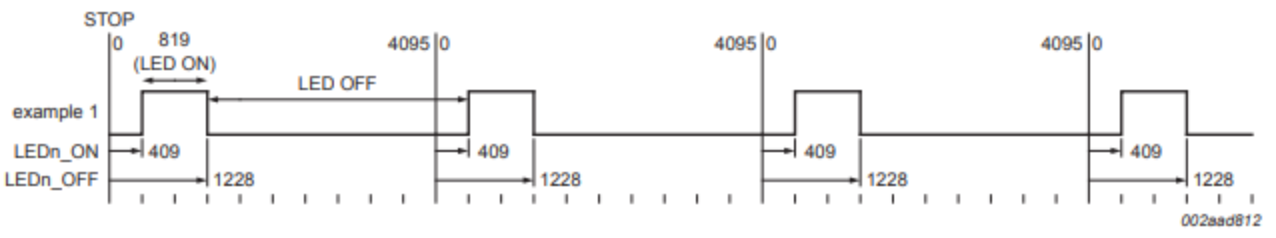
\includegraphics[width=\textwidth]{images/becker_esp_pca9685.png}
        \caption{Erklärung ON\slash OFF Parameter für PCA9685 aus \cite[S.~17]{esp_pca9685_datasheet}}
        \label{fig:esp_pca9685_on_off}
    \end{figure}

    \item \textbf{pca9685\_set\_off}: Mittels dieser Funktion kann das PWM-Signal auf einem bestimmten Kanal deaktiviert werden.
\end{itemize}

Auf Basis dieses Treiber wurden im nächsten Schritt zwei Interfaces programmiert: 
Einerseits das Interface zur Plattform-Kontrolle und andererseits das Interface zur Schusskontrolle, welches zusätzlich der Logik zur Ansteuerung der Flywheel-Motoren enthält.

\subsection{Ansteuerung der Servo-Motoren (Becker)}

Um nun die Plattform sowohl manuell über den DualShock4-Controller als auch semi-automatisch per künstlicher Intelligenz über MQTT präzise steuern zu können, wurde ein Interface entwickelt, das die Ansteuerung eines Motors an eine bestimmte Position erlaubt. 

In diesem Kontext wird mit der Einheit Grad gearbeitet. 
Ein Blick in die Referenz \cite{esp_servo_control} der Servo-Motoren zeigt, dass durch die Einstellung der Duty-Cycle-Länge des PWM-Signals eine Drehung auf eine bestimmte Grad-Position erreicht wird. 
Im ersten Schritt wurden die \textit{OFF} Werte für die Punkte \ang{-90} (max. Drehung nach links), \ang{0} und \ang{90} (max. Drehung nach rechts) manuell ermittelt.
Die absoluten Werte für die Drehungen werden im Folgenden als $value_{-90^\circ}$, $value_{0^\circ}$ und $value_{90^\circ}$ bezeichnet.

Für die Berechnung des Zielwerts $value_{off}$ für den \textit{OFF} Wert des PWM-Board-Treibers aus einem gegebenen Winkel wird Formel \ref{eq:pwm_to_duty} verwendet.

\begin{gather}
    \begin{aligned}
    &\text{Sei } \theta \text{ der gewünschte Winkel,} \\
    &|\theta| = \text{Betrag von } \theta \\
    &n_3 = \left\lfloor \frac{|\theta|}{3} \right\rfloor \\
    &n_2 = |\theta| - n_3 \\
    &s = 2 \cdot n_2 + 3 \cdot n_3 \\
    &\tilde{s} =
    \begin{cases}
    s, & \theta > 0 \\
    -s, & \theta \leq 0
    \end{cases} \\
    &value_{off} = value_{zero} + \tilde{s}
    \end{aligned}
    \label{eq:pwm_to_duty}
\end{gather}

Die Idee der Formel beruht auf der Tatsache, dass die Differenz aus $value_{90^\circ}$ bzw. $value_{-90^\circ}$ und $value_{0^\circ}$ gebildet und anschließend gleichmäßig auf den Bereich von $]1, 90[$, also auf 90 Werte, aufgeteilt wird. 

Für jedes zusätzliche Grad Rotation um den Nullpunkt müssten demnach entweder $2.\overline{3}$ addiert oder subtrahiert werden.
Da dies in Anbetracht der Verwendung von Festkommazahlen nicht realisierbar wäre, erscheint die naheliegende Idee, den Wert zu runden. 
Diese Praktik würde jedoch im Zeitverlauf zu einer zunehmenden Abweichung und folglich zu einem Verlust an Präzision führen.
Um das genannte Problem zu vermeiden, wird der \textit{OFF} Wert für jedes dritte Grad Drehung um den Faktor 3 verändert und für jedes andere Grad um Faktor 2.
Die Formel \ref{eq:pwm_to_duty} berechnet dabei in $n_3$ die Anzahl der Faktor-3-Drehungen und in $n_2$ die Anzahl der Faktor-2-Drehungen.
Ausgehend davon wird $value_{0^\circ}$ verändert.

Das Endergebnis stellt eine Funktion dar, mittels derer eine präzise gradweise Ansteuerung beider Plattformachsen möglich ist.

Darüber hinaus wurde im Interface ein Clipping der Werte als Sicherheitmechanismus integriert. Im Zuge der Initialisierung des Plattforminterfaces muss für jede Achse ein Startwinkel sowie ein linker und rechter Stopwinkel angegeben werden.
Sollte es bei der Steuerung durch den Dualshock4-Controller in dessen Regelschleife oder in der KI-Berechnung zu einem fehlerhaften Gradwert kommen, wird dieser Wert automatisch an den nächstgelegenen Stopwinkel geclippt. 
Durch diese Maßnahme werden potenzielle Materialschäden, die durch fehlerhafte Drehungen verursacht werden könnten, verhindert.

Die Realisierung der Ansteuerung des kleinen Servos, dessen Funktion darin besteht, die Nerf-Darts in die Flywheel-Motoren zu schieben, würde durch die Verwendung dieser Art der Ansteuerung zu einer unnötigen Komplexität führen.
Daher wurde für diesen Motor lediglich eine Startposition (Geschütztrigger ganz hinten; Dart kann in das Magazin fallen) und eine Endposition (Geschütztrigger ganz vorne; Dart wurde in die Flywheels geschoben) durch manuelles Einsetzen von \textit{OFF} Werten festgelegt.
Wird nun ein Schuss ausgelöst, so fährt der Servo-Motor zunächst in seine Endposition und von dort aus wieder zurück in seine Startposition.

\subsection{Ansteuerung der Flywheel Motoren (Becker, Koch, Wohlrab)}

Für die Vervollständigung des Fire-Control Interfaces wird nun noch die Ansteuerung der Flywheel-Motoren benötigt.
In dem vorliegenden Projekt erfolgt die Steuerung der beiden Gleichstrommotoren jeweils durch ein Power-MOSFET-Modul.

Die Funktionsweise des Modul lässt sich folgendermaßen beschreiben:

\begin{itemize}
    \item Auf einer Seite wird der Eingangstrom, in unserem Fall 5V, vom Stromverteiler eingeführt.
    \item Andererseits wird der Ausgang jeweils mit einem Motor verbunden.
    \item Die am Ausgang ausgegebene Spannung kann über einen PWM-Pin geregelt werden \cite{esp_platform_flywheel_motor}.
\end{itemize}

Die Wahl fiel auf dieses relativ simple Modul, da lediglich die Anforderung bestand, dass sich die Motoren bei der Schussabgabe möglichst schnell drehen sollen.
Im Rahmen dieses Projekts waren keine Änderungen der Richtung oder präzisere Steuerung erforderlich.

Im Rahmen des manuellen Tests wurde festgestellt, dass zur Erzielung eines optimalen Schussbildes eine Versorgung der Motoren mit 5 Volt erforderlich ist. 
Infolgedessen beträgt der Duty-Cycle entweder 0 oder 100 Prozent.
Daher wurde der ursprüngliche PWM-Code letztlich auf das reine Ein- und Ausschalten eines GPIO-Pins reduziert.

\section{Integration (Becker, Specht)}